\documentclass[10pt,letterpaper]{article}

\usepackage[T1]{fontenc}
\usepackage[utf8]{inputenc}
\usepackage{newtxtext,newtxmath}
\usepackage[letterpaper,margin=0.44in,top=0.40in,bottom=0.42in]{geometry}
\usepackage{microtype}
\usepackage{graphicx}
\usepackage{array}
\usepackage{booktabs}
\usepackage{tabularx}
\usepackage{enumitem}
\usepackage[table]{xcolor}
\usepackage{multicol}
\usepackage{fancyhdr}

\definecolor{TitoInk}{HTML}{17201B}
\definecolor{TitoRed}{HTML}{B72831}
\definecolor{TitoRule}{HTML}{59605C}
\definecolor{TitoPale}{HTML}{F2F1EC}
\definecolor{TitoBlue}{HTML}{DDE8E6}

\setlength{\parindent}{0pt}
\setlength{\parskip}{2.5pt}
\setlength{\columnsep}{0.24in}
\setlist{nosep}
\renewcommand{\arraystretch}{1.12}

\pagestyle{fancy}
\fancyhf{}
\fancyfoot[C]{\sffamily\scriptsize TITO PLAYER AID \textbullet\ \thepage}
\renewcommand{\headrulewidth}{0pt}
\setlength{\headheight}{12pt}

\newcommand{\aidheading}[1]{%
  \par\vspace{4pt}%
  {\sffamily\bfseries\large\color{TitoInk}#1\par}%
  \vspace{1.5pt}{\color{TitoRule}\hrule height 0.5pt}\vspace{4pt}%
}

\newcommand{\aidsubhead}[1]{%
  \par\vspace{3pt}{\sffamily\bfseries\color{TitoInk}#1\par}\vspace{1pt}%
}

\newcommand{\nationpic}[1]{\includegraphics[width=0.50in]{figures/#1.pdf}}

\newcommand{\stage}[1]{%
  \par\smallskip\noindent{\sffamily\bfseries\color{TitoInk}#1}\par%
}

\newcommand{\dash}{\textemdash}

\begin{document}
\thispagestyle{fancy}

\noindent
\begin{minipage}[t]{0.57\textwidth}
  {\sffamily\bfseries\fontsize{32}{32}\selectfont\color{TitoInk}TITO\par}
  \vspace{1pt}
  {\sffamily\bfseries\fontsize{17}{19}\selectfont\color{TitoRule}
    Player Aid\par}
\end{minipage}
\hfill
\begin{minipage}[t]{0.39\textwidth}
  \raggedleft\vspace{1pt}
  {\sffamily\bfseries Rules Reference\par}
  {\sffamily\small Version 1.0\par}
  {\sffamily\small \today\par}
\end{minipage}

\vspace{3pt}
{\color{TitoInk}\hrule height 1.2pt}
\vspace{3pt}

\begin{minipage}[t]{0.47\textwidth}
\vspace{0pt}
\aidheading{Terrain Key}
\begin{center}
  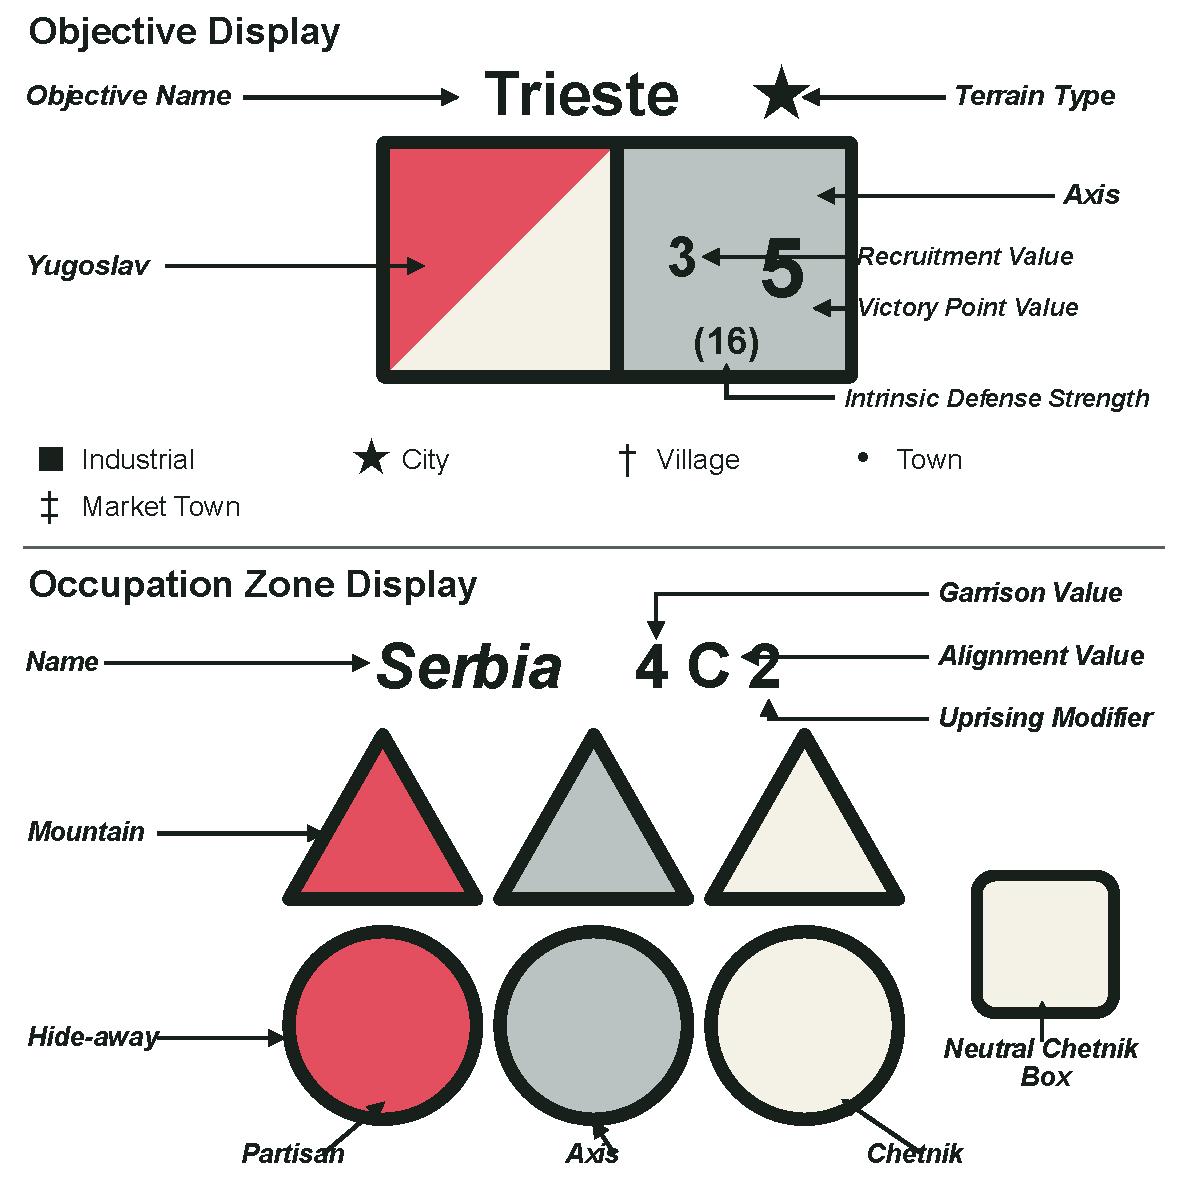
\includegraphics[width=0.98\linewidth]{figures/player-aid-terrain-key.pdf}
\end{center}

\aidheading{Unit Key}
\begin{center}
  {\sffamily\bfseries Axis Unit\par}
  \vspace{2pt}
  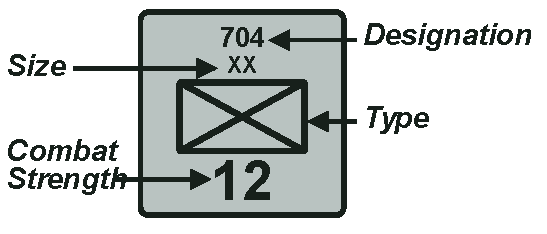
\includegraphics[width=0.98\linewidth]{figures/counter-anatomy.pdf}

  \vspace{4pt}
  {\sffamily\bfseries Partisan Unit\par}
  \vspace{2pt}
  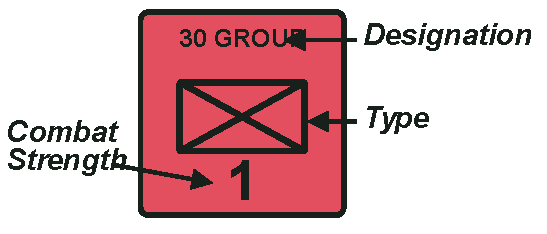
\includegraphics[width=0.98\linewidth]{figures/counter-anatomy-partisan-front.pdf}
\end{center}
\vspace{-2pt}

\footnotesize
\textbf{Size symbols:} II Battalion; III Regiment; X Brigade; XX Division;
XXX Corps. Guerrilla groups have no size symbol.
\end{minipage}
\hfill
\begin{minipage}[t]{0.50\textwidth}
\vspace{0pt}
\aidheading{Abbreviated Sequence of Play}
\small

\stage{A. Special Events Stage}
\begin{enumerate}[leftmargin=1.35em,label=\arabic*.,itemsep=1.4pt]
  \item \textbf{Allied Progress Phase} (Game-Turn 6 and after).
  \item \textbf{Weather Phase} (Game-Turns 2, 6, 10, and 14).
  \item \textbf{Tito Phase} (when eligible, through Game-Turn 14).
  \item \textbf{Axis Reinforcement Phase.}
  \item \textbf{Chetnik Collaboration Phase} (Game-Turns 2--17).
  \item \textbf{Italian Surrender Phase} (Game-Turn of surrender only).
  \item \textbf{Axis Anti-Guerrilla Operations Phase} (Game-Turns 3--14):
    \begin{enumerate}[leftmargin=1.35em,label=\alph*.,itemsep=0.5pt]
      \item Planning Segment
      \item Yugoslav Reaction Segment
      \item Deployment Segment
      \item Combat Segment
    \end{enumerate}
\end{enumerate}

\stage{B. Yugoslav Player-Turn}
\begin{enumerate}[leftmargin=1.35em,label=\arabic*.,itemsep=1pt]
  \item Movement Phase
  \item Combat Phase
\end{enumerate}

\stage{C. Victory Point Stage}

\stage{D. Axis Player-Turn}
\begin{enumerate}[leftmargin=1.35em,label=\arabic*.,itemsep=1pt]
  \item Movement Phase
  \item Combat Phase
\end{enumerate}

\stage{E. Terminal Stage}
\begin{enumerate}[leftmargin=1.35em,label=\arabic*.,itemsep=1.4pt]
  \item \textbf{Guerrilla Reinforcement Phase}
    \begin{enumerate}[leftmargin=1.35em,label=\alph*.,itemsep=0.5pt]
      \item Recruitment Segment
      \item Tito Segment
      \item Uprising Segment (Game-Turn 3 and after)
    \end{enumerate}
  \item Guerrilla Status Phase
  \item Axis Anti-Guerrilla Operations Redeployment Phase
  \item Game-Turn Indication Phase
\end{enumerate}

\vspace{5pt}
\colorbox{TitoPale}{%
  \parbox{\dimexpr\linewidth-2\fboxsep\relax}{%
    \footnotesize
    \textbf{Game-Turn 1:} Begin with the Yugoslav Player-Turn; skip the Special
    Events Stage. \quad
    \textbf{Game-Turn 17:} End after the Victory Point Stage; skip the Axis
    Player-Turn and Terminal Stage.}}

\aidheading{Quick Movement Reminders}
\footnotesize
\begin{itemize}[leftmargin=1.2em,itemsep=2pt]
  \item Axis units normally move through up to three contiguous Zones.
  \item Yugoslav units move within their current Zone or into one adjacent
    Zone, normally ending in a Mountain or Hide-away.
  \item Axis units may enter a Hide-away only during an Anti-Guerrilla
    Operation.
  \item A location may contain no more than seven divisions or equivalents at
    the end of a Movement Phase; guerrilla groups stack for free.
\end{itemize}

\aidheading{Nationality Colors}
\centering
\begin{tabular}{@{}c c c c@{}}
  \nationpic{german-infantry-front} &
  \nationpic{serbian-infantry} &
  \nationpic{italian-infantry} &
  \nationpic{croat-infantry} \\
  \footnotesize German & \footnotesize Serbian & \footnotesize Italian &
  \footnotesize Croat \\
  \addlinespace[3pt]
  \nationpic{bulgarian-infantry} &
  \nationpic{soviet-infantry} &
  \nationpic{partisan-group} &
  \nationpic{chetnik-group} \\
  \footnotesize Bulgarian & \footnotesize Soviet & \footnotesize Partisan &
  \footnotesize Chetnik
\end{tabular}
\end{minipage}

\clearpage

\noindent
{\sffamily\bfseries\fontsize{22}{23}\selectfont\color{TitoInk}
  TITO \textcolor{TitoRule}{Reference Tables}\par}
\vspace{2pt}
{\color{TitoInk}\hrule height 1.0pt}
\vspace{2pt}

\aidheading{[6.7] Occupation Zone Table}
\small
\textit{Game-Turn in which listed units may enter. Parenthetical entries refer
to the notes below.}

\vspace{3pt}
\begingroup
\footnotesize
\setlength{\tabcolsep}{3.7pt}
\rowcolors{2}{TitoBlue!48}{white}
\begin{tabularx}{\linewidth}{@{}>{\bfseries}l *{7}{>{\centering\arraybackslash}X}@{}}
  \rowcolor{TitoInk!15}
  Zone & German & Italian & Bulgarian & Croat & Serbian &
  \shortstack{Partisan/\\Chetnik} & Soviet \\
  Albania    & (c) & All & 16 & \dash & \dash & All & 16 \\
  Baranya    & 15  & \dash & 17 & \dash & \dash & 15 & 16 \\
  Bosnia     & All & (d) & 17 & All & \dash & All & 16 \\
  Carinthia  & 15  & \dash & \dash & \dash & \dash & 15 & \dash \\
  Croatia    & (c) & All (e) & 17 & All & \dash & All & 16 \\
  Dalmatia   & (c) & All & \dash & (g) & \dash & All & 17 \\
  Islands    & (c) & All & \dash & \dash & \dash & All & 17 \\
  Istria     & (c) & All & \dash & \dash & \dash & All & \dash \\
  Macedonia  & 15  & \dash & All & \dash & \dash & All (h) & 15 \\
  Montenegro & (c) & All & 16 & \dash & \dash & All & 16 \\
  Serbia     & All & (d) & (f) & \dash & All & All & 15 \\
  Slovenia   & (c) & All & \dash & \dash & \dash & All & \dash \\
\end{tabularx}
\endgroup

\vspace{4pt}
\begin{multicols}{2}
\small
\textbf{Key.} ``All'' means the unit may enter on every Game-Turn, subject to
the notes and normal movement rules. A dash means the unit may never enter.

\textbf{(a)} On Game-Turns 1 and 2, all units remain in the Zone where they
start or enter as reinforcements (6.63).

\textbf{(b)} Soviet and pro-Yugoslav Bulgarian reinforcement placement is
specified in 13.92.

\textbf{(c)} German units may enter the Italian sphere after the Yugoslav
Player first reaches 45 Victory Points or places the first Yugoslav brigade
(6.64A).

\columnbreak
\textbf{(d)} After that same trigger, up to three Italian divisions may enter
Serbia or Bosnia during an Anti-Guerrilla Operation. They may not do so after
Italian Pullback and must redeploy into Croatia (6.64B).

\textbf{(e)} Subject to Italian Pullback (10.2).

\textbf{(f)} After the trigger in 6.64, the Bulgarian 25th and 27th Divisions
may enter designated Bulgarian Occupation boxes in Serbia and may conduct an
Anti-Guerrilla Operation there (6.64C).

\textbf{(g)} Croat units may enter Dalmatia after Italian Surrender (6.66).

\textbf{(h)} Through Game-Turn 13, Macedonia may contain no more than four
Partisan and four Chetnik units of any allegiance (6.67).
\end{multicols}

\aidheading{[8.6] Combat Results Table}
\begingroup
\footnotesize
\setlength{\tabcolsep}{3.0pt}
\renewcommand{\arraystretch}{1.32}
\rowcolors{2}{TitoBlue!55}{white}
\begin{tabularx}{\linewidth}{@{}>{\bfseries}c *{13}{>{\centering\arraybackslash}X}@{}}
  \rowcolor{TitoInk!15}
  Die & 1:2 & 1:1 & 2:1 & 3:1 & 4:1 & 5:1 & 6:1 & 7:1 & 8:1 & 9:1 &
  10:1 & 11:1 & 12:1 \\
  1 & Ae & Ae & A4 & A3 & A2 & A1 & D1 & D1 & D1 & D2 & D3 & D4 & De \\
  2 & Ae & A4 & A3 & A2 & A1 & D1 & D1 & D1 & D2 & D3 & D4 & De & De \\
  3 & A4 & A3 & A2 & A1 & D1 & D1 & D1 & D2 & D3 & D4 & De & De & De \\
  4 & A3 & A2 & A1 & D1 & D1 & D1 & D2 & D3 & D4 & De & De & De & De \\
  5 & A2 & A1 & D1 & D1 & D1 & D2 & D3 & D4 & De & De & De & De & De \\
  6 & A1 & D1 & D1 & D1 & D2 & D3 & D4 & De & De & De & De & De & De \\
\end{tabularx}
\endgroup

\vspace{5pt}
\begin{multicols}{2}
\small
\aidsubhead{Results}
\textbf{Ae/De:} The entire attacking or defending force is eliminated.

\textbf{A\#/D\#:} The affected force loses units totaling as many Strength
Points as possible without exceeding the number, then retreats. Attacks below
1:2 use the 1:2 column; attacks above 12:1 use the 12:1 column.

\aidsubhead{Terrain and Numerical Losses}
\begin{itemize}[leftmargin=1.2em,itemsep=1pt]
  \item Hide-away defenders are doubled in Combat Strength.
  \item Triple a numerical result in a city.
  \item Double it in a town or market town.
  \item Double it during an Anti-Guerrilla Operation.
\end{itemize}

\columnbreak
\aidsubhead{Ratio-Column Shifts}
\begin{itemize}[leftmargin=1.2em,itemsep=1.5pt]
  \item \textbf{Mountain unit:} shift one column right when a German or Italian
    mountain unit attacks a Mountain, Hide-away, or village; maximum one shift.
  \item \textbf{Tito participates:} shift one column right in a Partisan attack
    or one column left in a Partisan defense.
  \item \textbf{Anti-Guerrilla Operation:} shift two columns right.
  \item \textbf{After Tito is eliminated:} shift one column right for Axis
    attacks against Partisans and one column left for Partisan attacks.
\end{itemize}
\end{multicols}

\vfill
\colorbox{TitoPale}{%
  \parbox{\dimexpr\linewidth-2\fboxsep\relax}{%
    \small
    \textbf{Combat procedure:} Total participating Strength Points
    $\rightarrow$ apply defensive terrain effects $\rightarrow$ form and round
    down the attacker:defender ratio $\rightarrow$ apply ratio shifts
    $\rightarrow$ roll one die $\rightarrow$ apply and modify the result
    $\rightarrow$ retreat if required.}}

\end{document}
